\documentclass{article}
\usepackage{xcolor}
\definecolor{BLUELINK}{HTML}{0645AD}
\definecolor{DARKBLUELINK}{HTML}{0B0080}
\definecolor{LIGHTBLUELINK}{HTML}{3366BB}
\definecolor{PURPLELINK}{HTML}{663366}
\PassOptionsToPackage{hyphens}{url}
\usepackage[colorlinks=false ]{hyperref}
% for linking between references, figures, TOC, etc in the pdf document
\hypersetup{colorlinks,
linkcolor=DARKBLUELINK,
anchorcolor=DARKBLUELINK,
citecolor=DARKBLUELINK,
filecolor=DARKBLUELINK,
menucolor=DARKBLUELINK,
urlcolor=BLUELINK
} % Color citation links in purple
\PassOptionsToPackage{unicode}{hyperref}
\PassOptionsToPackage{naturalnames}{hyperref}

\usepackage[margin=60pt]{geometry}
\usepackage{amssymb,amsfonts,amsmath,amsthm,mathtools}
\usepackage{lmodern}
\usepackage{bm,bbold}
\usepackage{verbatim}
\usepackage{float}
\usepackage{listings, enumerate, enumitem}
\usepackage[export]{adjustbox}
\usepackage{tabu}
\tabulinesep=0.6mm
\newcommand\cellwidth{\TX@col@width}
\usepackage{hhline}
\setlength{\arrayrulewidth}{1.2pt}
\usepackage{multicol,multirow,array}
\usepackage{etoolbox}
\AtBeginEnvironment{tabu}{\footnotesize}
\usepackage{booktabs}

\usepackage{graphicx}
\graphicspath{{artworks/}}
\makeatletter
\def\input@path{{artworks/}}
\makeatother
\pdfstringdefDisableCommands{%
\renewcommand*{\bm}[1]{#1}%
% any other necessary redefinitions
}
\usepackage{xfrac, nicefrac}
\usepackage{natbib}
\pdfinclusioncopyfonts=1
\definecolor{RED}{HTML}{EB6231}
\definecolor{YELLOW}{HTML}{E29D26}
\definecolor{BLUE}{HTML}{5D80B4}
\definecolor{LIGHTGREEN}{HTML}{6ABD9B}
\definecolor{GREEN}{HTML}{8FB03E}
\definecolor{PURPLE}{HTML}{BE1E2D}
\definecolor{BROWN}{HTML}{A97C50}
\definecolor{PINK}{HTML}{DA1C5C}

\newcommand{\der}{\mathrm{d}}
\newcommand{\e}{\mathrm{e}}
\newcommand{\dnds}{dNdS}
\newcommand{\indice}{l}
\newcommand{\indiceexp}{^{(\indice)}}
% Time, effective population size and mutation rate.
\newcommand{\Ne}{N}
% \acrshort{DNA}
\newcommand{\SetNuc}{\Omega_{\mathrm{N}}}
\newcommand{\SetWeak}{\Omega_{\mathrm{W}}}
\newcommand{\SetStrong}{\Omega_{\mathrm{S}}}
\newcommand{\mutmatrix}{R}
\newcommand{\Mutmatrix}{\bm{\mutmatrix}_{4\times4}}
\newcommand{\exchan}{\rho}
\newcommand{\Exchan}{\bm{\exchan}_{6\times1}}
\newcommand{\mutequi}{\sigma}
\newcommand{\Mutequi}{\bm{\mutequi}_{4\times1}}
% Codons
\newcommand{\SetCodon}{\Omega_{\mathrm{C}}}
\newcommand{\ci}{{i}}
\newcommand{\cj}{{j}}
\newcommand{\itoj}{\ci, \cj}
\newcommand{\nucitoj}{\mathcal{M}(\itoj)}
\newcommand{\submatrix}{Q}
\newcommand{\Submatrix}{\bm{\submatrix}_{61\times61}}
\newcommand{\subequi}{\pi}
\newcommand{\Subequi}{\bm{\subequi}_{61\times1}}
\newcommand{\probmatrix}{P}
\newcommand{\Probmatrix}{\bm{\probmatrix}_{61\times61}}
% Amino-acids
\newcommand{\SetAa}{\Omega_{\mathrm{A}}}
\newcommand{\Neighbor}{\mathcal{V}}
\newcommand{\NonSyn}{\mathcal{N}}
\newcommand{\Syn}{\mathcal{S}}
\newcommand{\Nx}{\Neighbor_x}
\newcommand{\NxAB}{\Neighbor_x^{\mathrm{A} \rightarrow \mathrm{B}}}
\newcommand{\NyBA}{\Neighbor_x^{\mathrm{B} \rightarrow \mathrm{A}}}
\newcommand{\NxWS}{\Neighbor_x^{\mathrm{W} \rightarrow \mathrm{S}}}
\newcommand{\NxSS}{\Neighbor_x^{\mathrm{S} \rightarrow \mathrm{S}}}
\newcommand{\NxSW}{\Neighbor_x^{\mathrm{S} \rightarrow \mathrm{W}}}
\newcommand{\NxWW}{\Neighbor_x^{\mathrm{W} \rightarrow \mathrm{W}}}
\newcommand{\NyWS}{\Neighbor_y^{\mathrm{W} \rightarrow \mathrm{S}}}
\newcommand{\NySS}{\Neighbor_y^{\mathrm{S} \rightarrow \mathrm{S}}}
\newcommand{\NySW}{\Neighbor_y^{\mathrm{S} \rightarrow \mathrm{W}}}
\newcommand{\NyWW}{\Neighbor_y^{\mathrm{W} \rightarrow \mathrm{W}}}
\newcommand{\NxNonSyn}{\NonSyn_x}
\newcommand{\NyNonSyn}{\NonSyn_y}
\newcommand{\NxSyn}{\Syn_x}
\newcommand{\NySyn}{\Syn_y}
\newcommand{\aminoacid}{\text{A}}
\newcommand{\aai}{\mathcal{A}(\ci)}
\newcommand{\aaj}{\mathcal{A}(\cj)}
\newcommand{\Ni}{\mathcal{N}_{\mathrm{eighbors}}\left(\ci\right)}
\newcommand{\NiNonSyn}{\mathcal{N}_{\mathrm{onSyn}}\left(\ci\right)}
\newcommand{\NiSyn}{\mathcal{S}_{\mathrm{yn}}\left(\ci\right)}
\newcommand{\fit}{f}
\newcommand{\Fit}{\bm{\fit}_{20\times1}}
\newcommand{\fiti}{\fit_{\aai}}
\newcommand{\fitj}{\fit_{\aaj}}
\newcommand{\scaledfit}{F}
\newcommand{\ScaledFit}{\bm{\scaledfit}_{20\times1}}
\newcommand{\scaledfiti}{\scaledfit_{\aai}}
\newcommand{\scaledfitj}{\scaledfit_{\aaj}}
\newcommand{\selcoef}{{\delta_{\fit}}}
\newcommand{\scaledselcoef}{{\Delta \scaledfit}}
% Tree
\newcommand{\Tree}{\mathcal{T}}
\newcommand{\node}{\text{v}}
\newcommand{\taxon}{\node}
\newcommand{\Settaxon}{1 \leq \taxon \leq \Ntaxa}
\newcommand{\Ntaxa}{P}
\newcommand{\treeroot}{0}
\newcommand{\treerootexp}{^{(\treeroot)}}
\newcommand{\branch}{\text{w}}
\newcommand{\branchexp}{^{(\branch)}}
\newcommand{\Nbranch}{2 \Ntaxa - 2}
\newcommand{\Setbranch}{1 \leq \branch \leq 2 \Ntaxa - 2}
\newcommand{\up}{\branch^{\uparrow}}
\newcommand{\down}{\node}
\newcommand{\nodeexp}{^{(\node)}}
\newcommand{\Nnode}{2 \Ntaxa - 2}
\newcommand{\Ninternal}{\Ntaxa - 2}
\newcommand{\Setnode}{\treeroot \leq \node \leq 2 \Ntaxa - 2}
\newcommand{\Setnodenoroot}{1 \leq \node \leq 2 \Ntaxa - 2}
\newcommand{\Setinternal}{\Ntaxa + 1 \leq \node \leq 2 \Ntaxa - 2}
\newcommand{\branchnode}{\mathcal{W}}
\newcommand{\age}{T}
\newcommand{\branchtime}{\Delta \age}
\newcommand{\branchlength}{L}
% Alignment
\newcommand{\data}{{\color{PINK}{D}}}
\newcommand{\Data}{\bm{\data}}
\newcommand{\site}{\text{s}}
\newcommand{\siteexp}{^{(\site)}}
\newcommand{\Nsite}{\text{N}_{\site}}
\newcommand{\Setsite}{1 \leq \site \leq \Nsite}
\newcommand{\branchsiteexp}{^{(\branch, \site)}}
\newcommand{\treerootsiteexp}{^{(\treeroot, \site)}}
\newcommand{\taxonsiteexp}{^{(\taxon, \site)}}
% Categories
\newcommand{\cat}{\text{k}}
\newcommand{\catVar}{\mathcal{K}}
\newcommand{\catexp}{^{(\cat)}}
\newcommand{\Ncat}{\text{N}_{\cat}}
\newcommand{\Setcat}{1 \leq \cat \leq \Ncat}
\newcommand{\catsite}{\catVar^{\left(\site\right)}}
\newcommand{\branchcatexp}{^{(\branch, \cat)}}
\newcommand{\treerootcatexp}{^{(\treeroot, \cat)}}
% Polymorphism
\newcommand{\copies}{\text{n}}
\newcommand{\samples}{\text{N}_{\copies}}
% Random variables
\newcommand{\pruning}{\psi}
\newcommand{\uniform}{0, 1}
\newcommand{\Identitymatrix}{\bm{I}_{2\times2}}
\newcommand{\brownian}{\bm{B}_{2\times1}}
\newcommand{\contrast}{\bm{C}_{2\times1}}
\newcommand{\Covariancematrix}{\bm{\varSigma}_{2\times2}}
\newcommand{\covariancedf}{q}
\newcommand{\covariancekappa}{\kappa}
\newcommand{\Scattermatrix}{\bm{A}_{2\times2}}
\newcommand{\Multivariate}{\bm{Z}_{2\times1}}
\newcommand{\base}{\varPi}
\newcommand{\Base}{\bm{\base}_{20\times1}}
\newcommand{\baseconc}{\alpha}
\newcommand{\Basecenter}{\bm{\gamma}_{20\times1}}
\newcommand{\stickbreaking}{\varOmega}
\newcommand{\StickBreaking}{\bm{\stickbreaking}_{\Ncat\times1}}
\newcommand{\stick}{\varPhi}
\newcommand{\stickbreakinghyper}{\beta}
% Mapping
\newcommand{\history}{\mathcal{H}}
\newcommand{\sn}{{\color{BLUE}{S}}}
\newcommand{\s}{{\color{LIGHTGREEN}{S_0^{k}}}}
\newcommand{\si}{{\color{PINK}{S_1^{k}}}}
\newcommand{\sii}{{\color{PINK}{S_2^{k}}}}
\newcommand{\siii}{{\color{PINK}{S_3^{k}}}}
\newcommand{\siiii}{{\color{PINK}{S_4^{k}}}}
\newcommand{\siiiii}{{\color{LIGHTGREEN}{S_5^{k}}}}


\begin{document}
\part*{Supplementary materials}
\tableofcontents
 
\vspace*{1cm}

\section{Simulated alignments}

\subsection{Mammalian phylogeny - 4980 codons}

\begin{figure}[!htb]
    \centering
    \begin{minipage}{0.325\linewidth}
        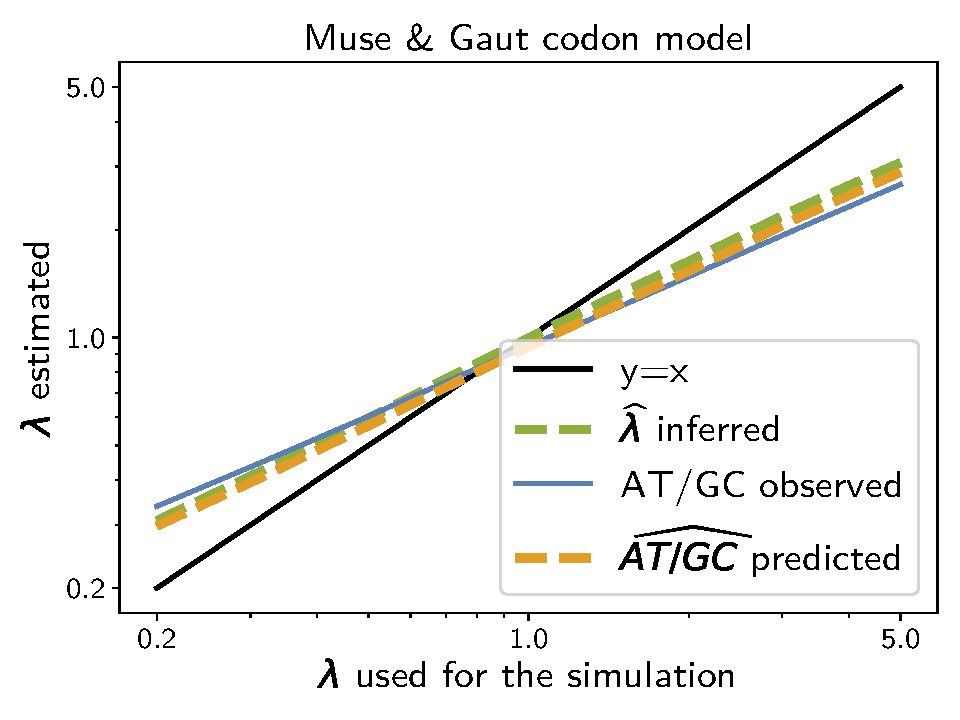
\includegraphics[width=\linewidth, page=1]{inference_supp_mat/MammalsExons10Mu1.0_lambda_MG.pdf}
    \end{minipage}
    \llap{\raisebox{1.25cm}{\scriptsize A\hspace{4.35cm}}}\hfill
    \begin{minipage}{0.325\linewidth}
        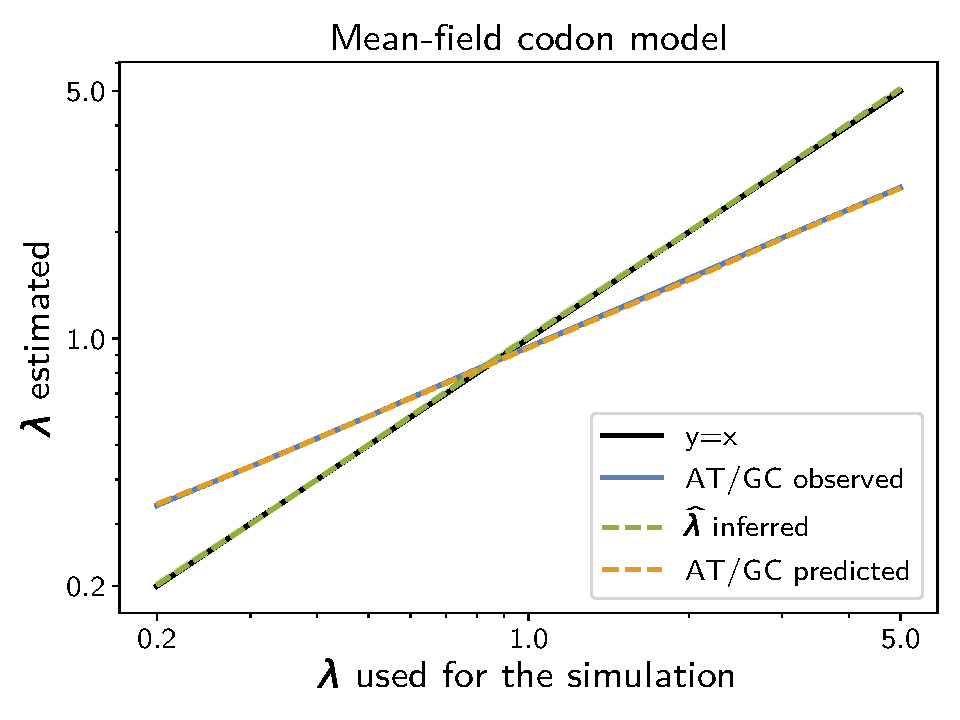
\includegraphics[width=\linewidth, page=1]{inference_supp_mat/MammalsExons10Mu1.0_lambda_MF.pdf}
    \end{minipage}
    \llap{\raisebox{1.25cm}{\scriptsize B\hspace{4.35cm}}}\hfill
    \begin{minipage}{0.325\linewidth}
        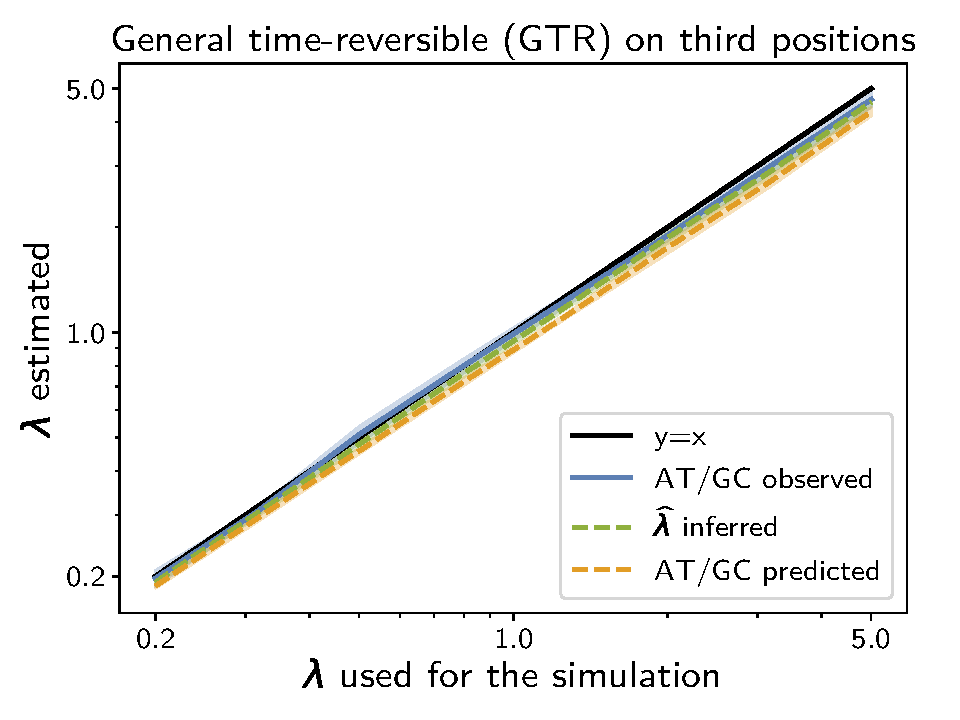
\includegraphics[width=\linewidth, page=1]{inference_supp_mat/MammalsExons10Mu1.0_lambda_GTR.pdf}
    \end{minipage}
    \llap{\raisebox{1.25cm}{\scriptsize C\hspace{4.35cm}}}\hfill
    \caption[Estimation of mutational bias]{
        Simulations for 90 mammalian taxa and 4980 codon sites.
        Estimated versus true mutational bias (bottom), using a codon model in which $\omega$ is modeled as a scalar (Muse \& Gaut formalism, MG, panel A) or as a tensor (mean-field approach, panel B), or by applying a GTR nucleotide model to the 4-fold degenerate third-coding positions only (panel C).
    }
\end{figure}

\subsection{Primate phylogeny - 2490 codons}

\begin{figure}[!htb]
    \centering
    \begin{minipage}{0.325\linewidth}
        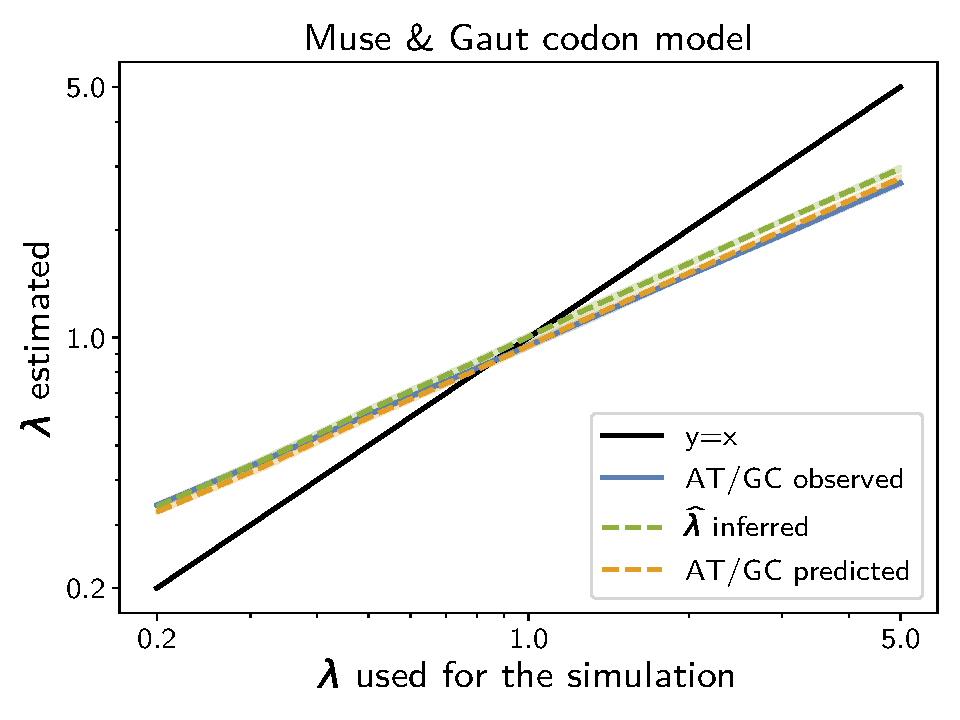
\includegraphics[width=\linewidth, page=1]{inference_supp_mat/PrimatesExons5Mu1.0_lambda_MG.pdf}
    \end{minipage}
    \llap{\raisebox{1.25cm}{\scriptsize A\hspace{4.35cm}}}\hfill
    \begin{minipage}{0.325\linewidth}
        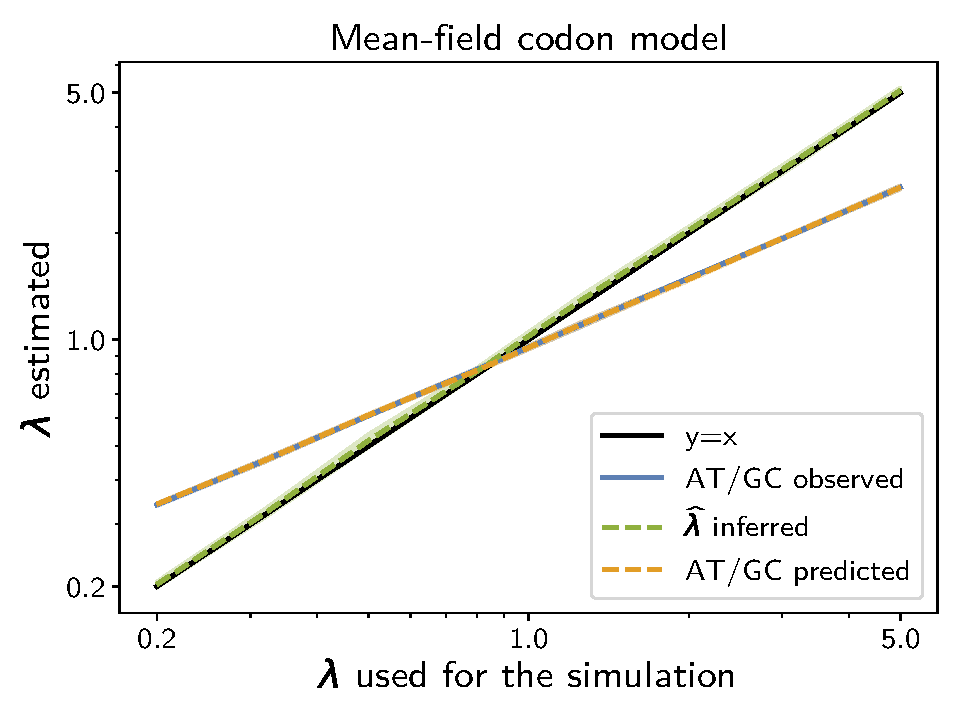
\includegraphics[width=\linewidth, page=1]{inference_supp_mat/PrimatesExons5Mu1.0_lambda_MF.pdf}
    \end{minipage}
    \llap{\raisebox{1.25cm}{\scriptsize B\hspace{4.35cm}}}\hfill
    \begin{minipage}{0.325\linewidth}
        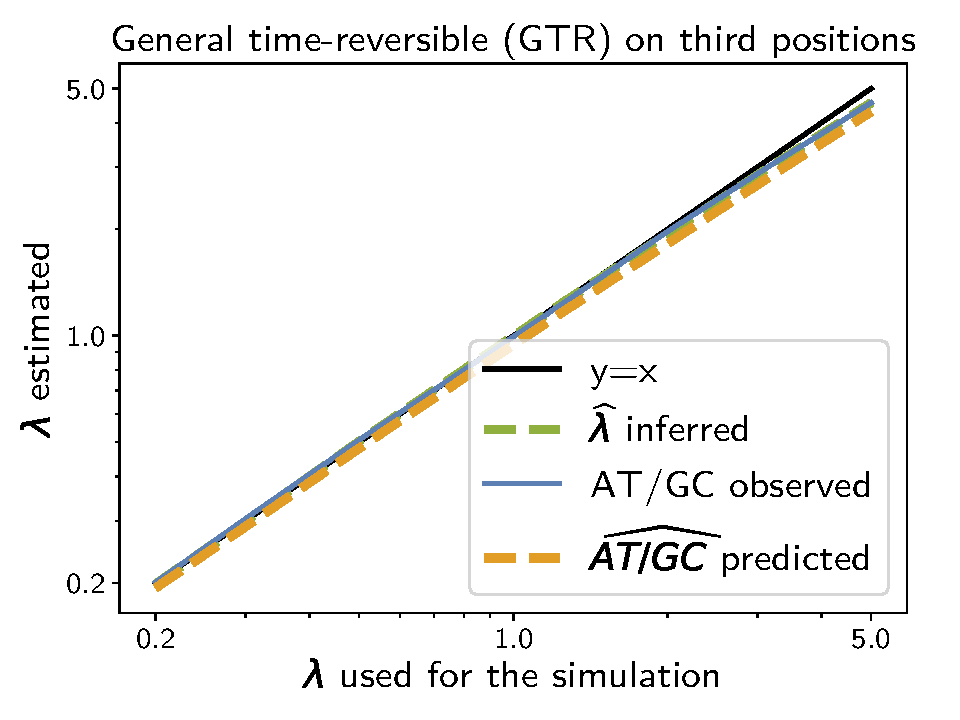
\includegraphics[width=\linewidth, page=1]{inference_supp_mat/PrimatesExons5Mu1.0_lambda_GTR.pdf}
    \end{minipage}
    \llap{\raisebox{1.25cm}{\scriptsize C\hspace{4.35cm}}}\hfill
    \caption[Estimation of mutational bias]{
        Simulations for 61 primate taxa and 2490 codon sites.
        Estimated versus true mutational bias (bottom), using a codon model in which $\omega$ is modeled as a scalar (Muse \& Gaut formalism, MG, panel A) or as a tensor (mean-field approach, panel B), or by applying a GTR nucleotide model to the 4-fold degenerate third-coding positions only (panel C).
    }
\end{figure}

\subsection{Primate phylogeny - 9960 codons}

\begin{figure}[!htb]
    \centering
    \begin{minipage}{0.325\linewidth}
        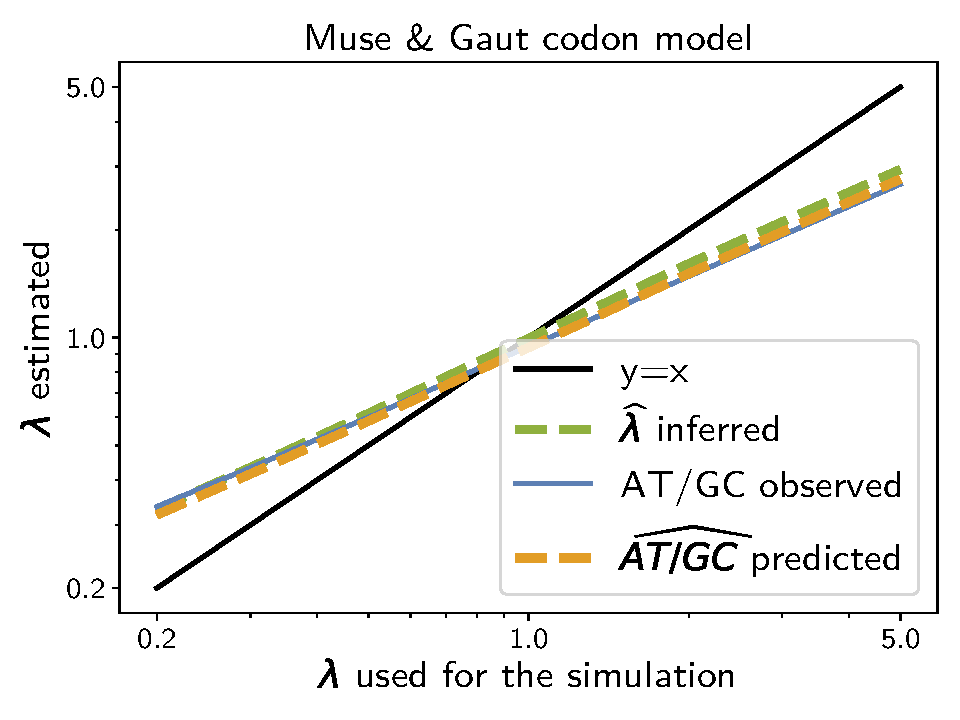
\includegraphics[width=\linewidth, page=1]{inference_supp_mat/PrimatesExons20Mu1.0_lambda_MG.pdf}
    \end{minipage}
    \llap{\raisebox{1.25cm}{\scriptsize A\hspace{4.35cm}}}\hfill
    \begin{minipage}{0.325\linewidth}
        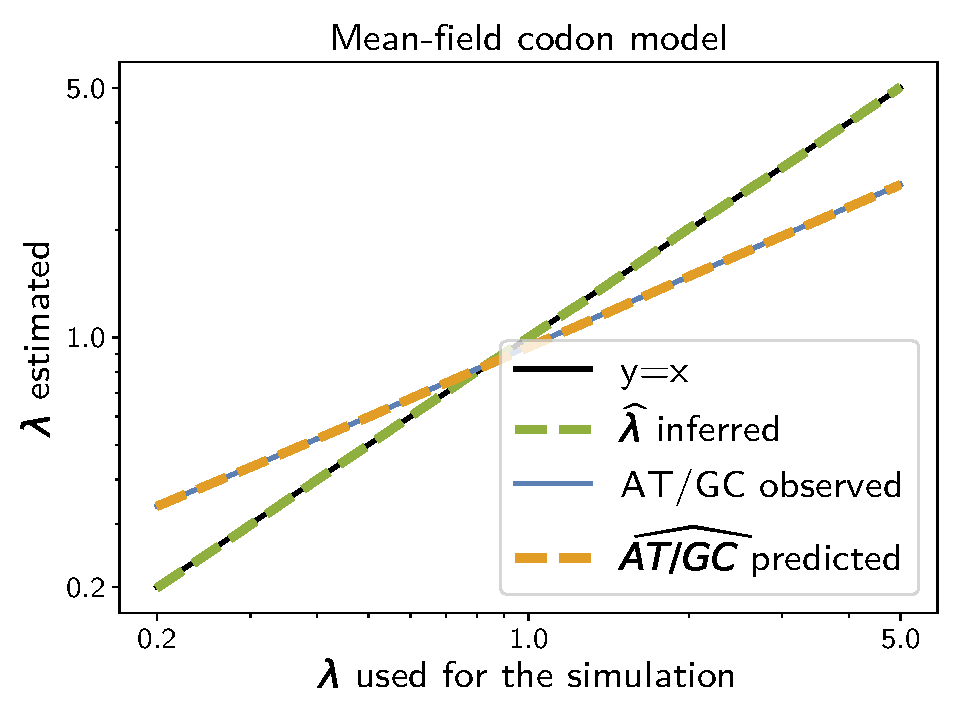
\includegraphics[width=\linewidth, page=1]{inference_supp_mat/PrimatesExons20Mu1.0_lambda_MF.pdf}
    \end{minipage}
    \llap{\raisebox{1.25cm}{\scriptsize B\hspace{4.35cm}}}\hfill
    \begin{minipage}{0.325\linewidth}
        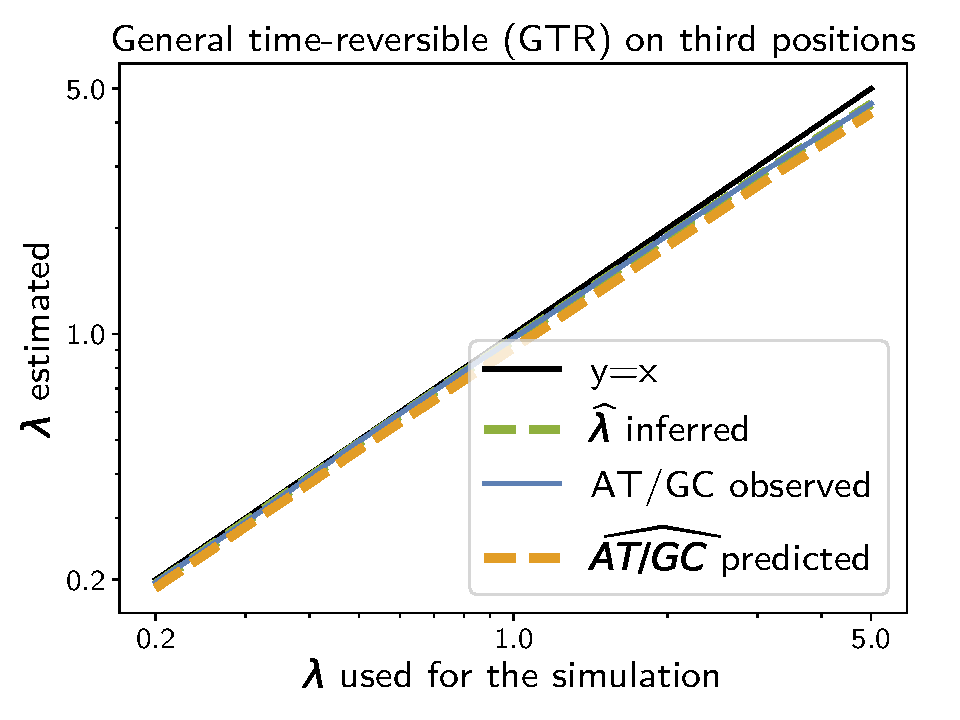
\includegraphics[width=\linewidth, page=1]{inference_supp_mat/PrimatesExons20Mu1.0_lambda_GTR.pdf}
    \end{minipage}
    \llap{\raisebox{1.25cm}{\scriptsize C\hspace{4.35cm}}}\hfill
    \caption[Estimation of mutational bias]{
        Simulations for 61 primate taxa and 9960 codon sites.
        Estimated versus true mutational bias (bottom), using a codon model in which $\omega$ is modeled as a scalar (Muse \& Gaut formalism, MG, panel A) or as a tensor (mean-field approach, panel B), or by applying a GTR nucleotide model to the 4-fold degenerate third-coding positions only (panel C).
    }
\end{figure}

\subsection{Primate phylogeny - 4980 codons - branch length x2}

\begin{figure}[!htb]
    \centering
    \begin{minipage}{0.325\linewidth}
        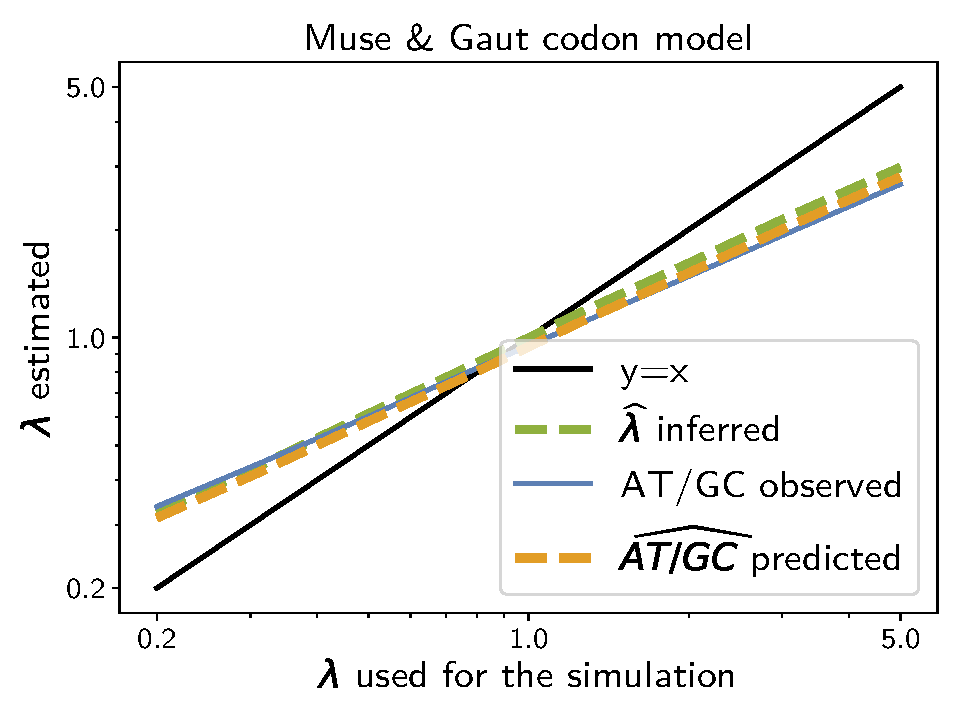
\includegraphics[width=\linewidth, page=1]{inference_supp_mat/PrimatesExons10Mu2.0_lambda_MG.pdf}
    \end{minipage}
    \llap{\raisebox{1.25cm}{\scriptsize A\hspace{4.35cm}}}\hfill
    \begin{minipage}{0.325\linewidth}
        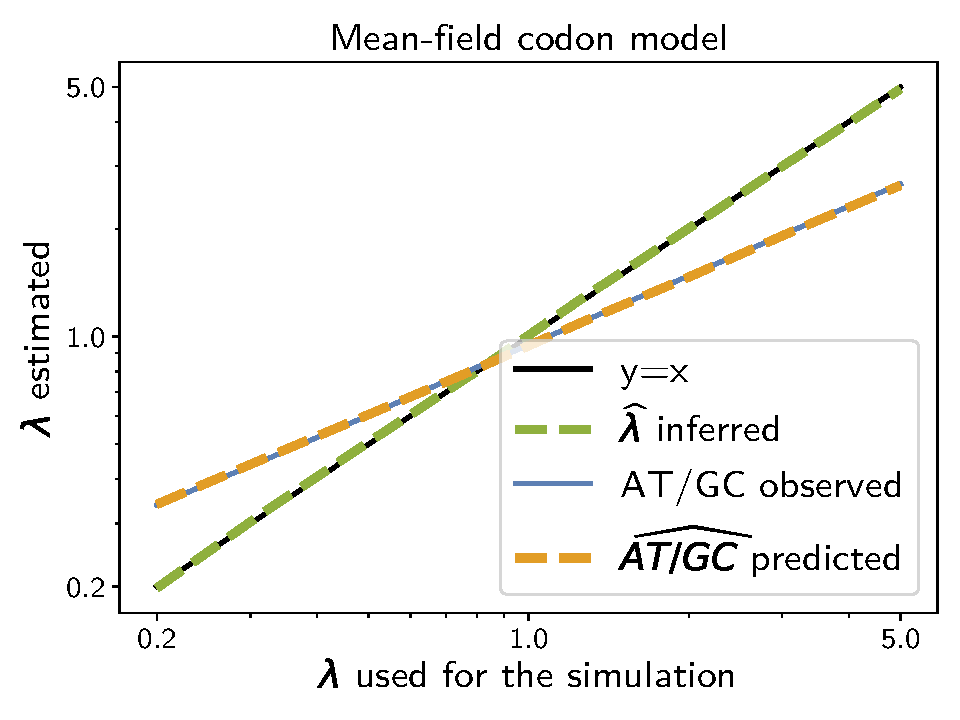
\includegraphics[width=\linewidth, page=1]{inference_supp_mat/PrimatesExons10Mu2.0_lambda_MF.pdf}
    \end{minipage}
    \llap{\raisebox{1.25cm}{\scriptsize B\hspace{4.35cm}}}\hfill
    \begin{minipage}{0.325\linewidth}
        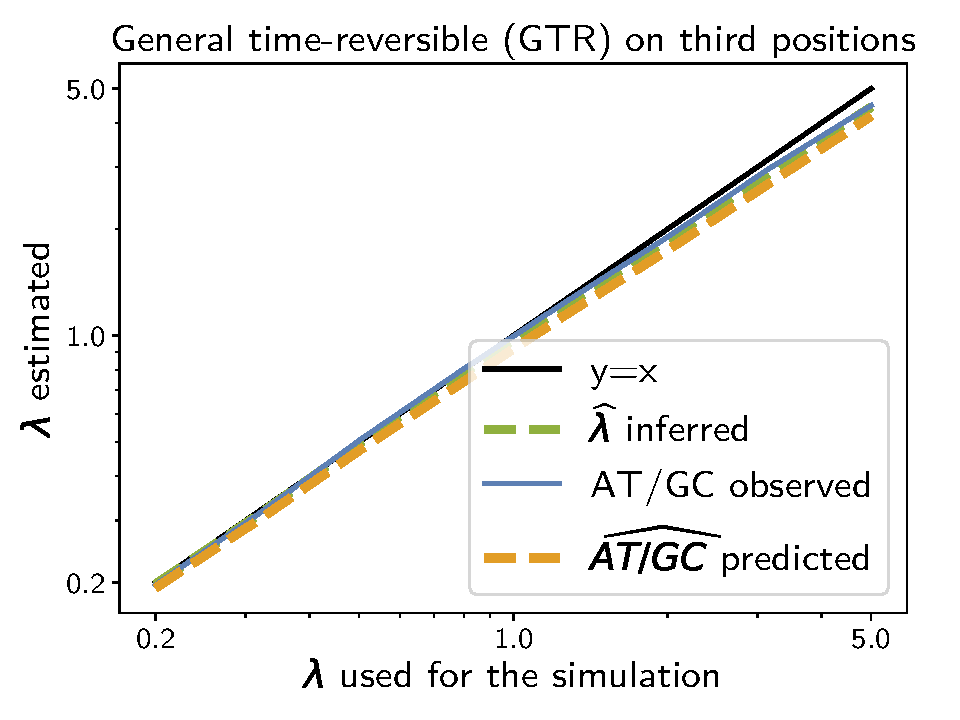
\includegraphics[width=\linewidth, page=1]{inference_supp_mat/PrimatesExons10Mu2.0_lambda_GTR.pdf}
    \end{minipage}
    \llap{\raisebox{1.25cm}{\scriptsize C\hspace{4.35cm}}}\hfill
    \caption[Estimation of mutational bias]{
        Simulations for 61 primate taxa with increased branch lenght by a factor 2 and 4980 codon sites.
        Estimated versus true mutational bias (bottom), using a codon model in which $\omega$ is modeled as a scalar (Muse \& Gaut formalism, MG, panel A) or as a tensor (mean-field approach, panel B), or by applying a GTR nucleotide model to the 4-fold degenerate third-coding positions only (panel C).
    }
\end{figure}

\subsection{Primate phylogeny - 4980 codons - branch length \%2}

\begin{figure}[!htb]
    \centering
    \begin{minipage}{0.325\linewidth}
        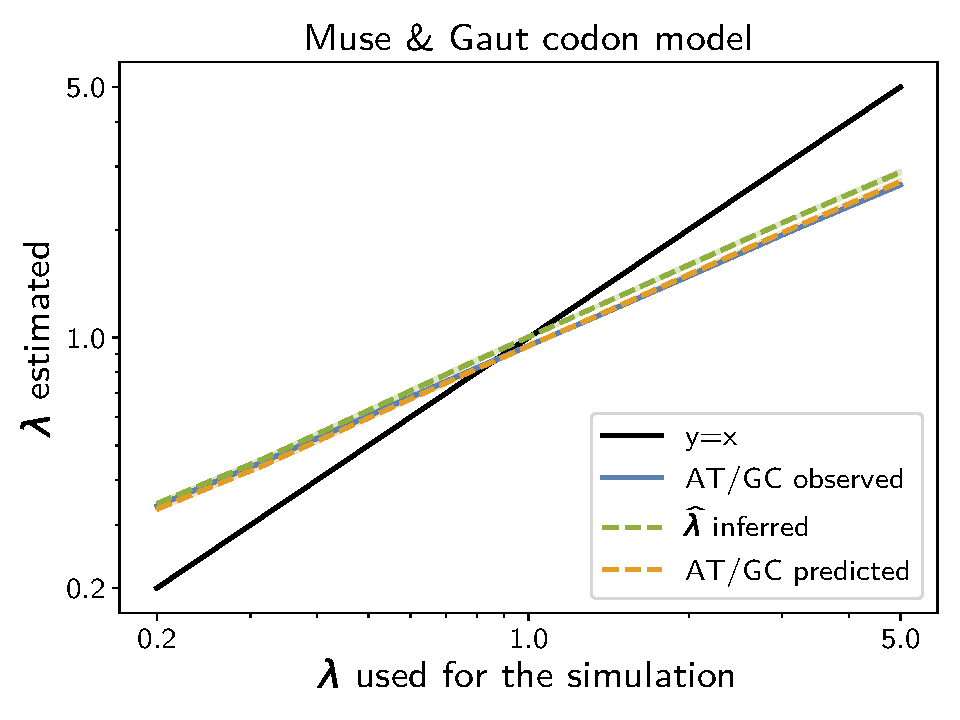
\includegraphics[width=\linewidth, page=1]{inference_supp_mat/PrimatesExons10Mu0.5_lambda_MG.pdf}
    \end{minipage}
    \llap{\raisebox{1.25cm}{\scriptsize A\hspace{4.35cm}}}\hfill
    \begin{minipage}{0.325\linewidth}
        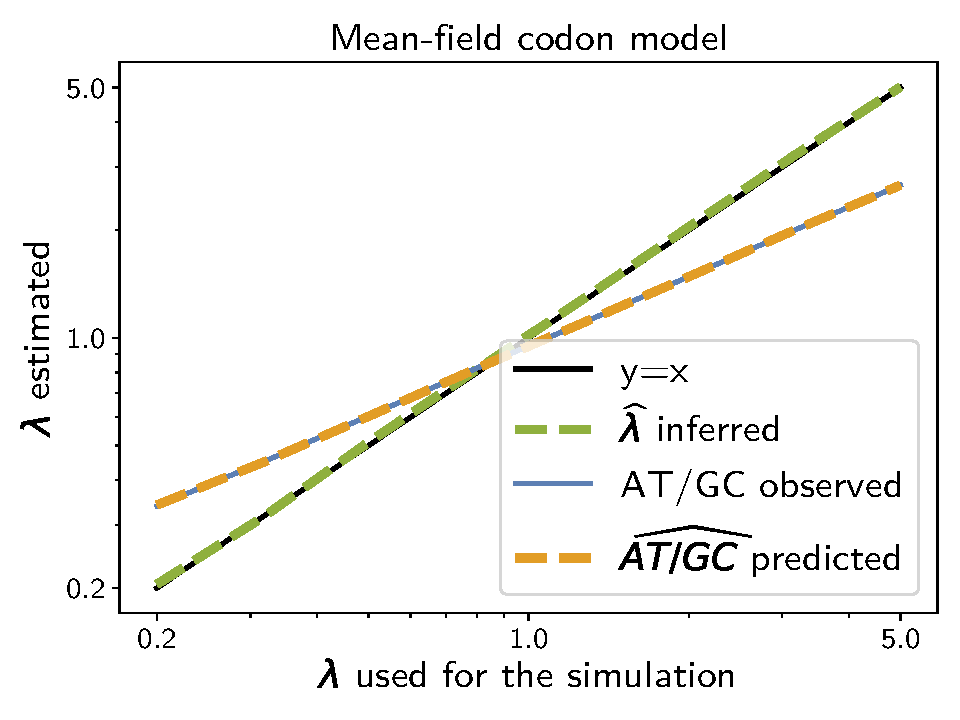
\includegraphics[width=\linewidth, page=1]{inference_supp_mat/PrimatesExons10Mu0.5_lambda_MF.pdf}
    \end{minipage}
    \llap{\raisebox{1.25cm}{\scriptsize B\hspace{4.35cm}}}\hfill
    \begin{minipage}{0.325\linewidth}
        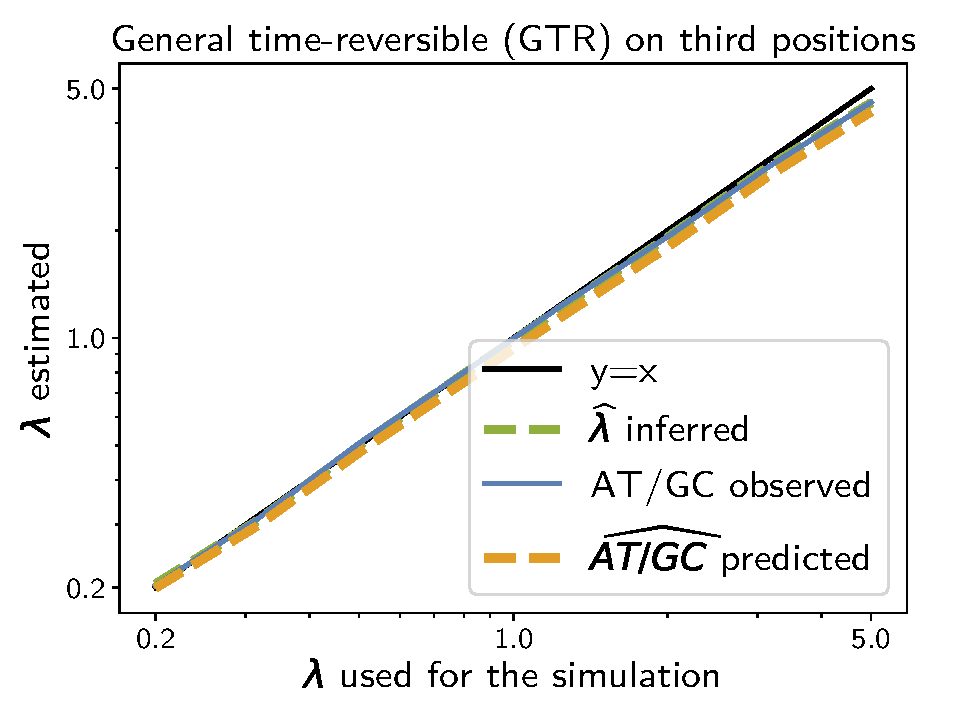
\includegraphics[width=\linewidth, page=1]{inference_supp_mat/PrimatesExons10Mu0.5_lambda_GTR.pdf}
    \end{minipage}
    \llap{\raisebox{1.25cm}{\scriptsize C\hspace{4.35cm}}}\hfill
    \caption[Estimation of mutational bias]{
        Simulations for 61 primate taxa with decreased branch lenght by a factor 2 and 4980 codon sites.
        Estimated versus true mutational bias (bottom), using a codon model in which $\omega$ is modeled as a scalar (Muse \& Gaut formalism, MG, panel A) or as a tensor (mean-field approach, panel B), or by applying a GTR nucleotide model to the 4-fold degenerate third-coding positions only (panel C).
    }
\end{figure}

\end{document}